\parhead{Extensive margin}

\noindent \underline{\textit{Specification 1: Recall}} \\[0.4em]
It appears that shared origin raises recall mostly because those specific ties were imported. Sharing a woreda increases the recall probability by \pnChanRecallOriginPp{} percentage points on a base recall rate of \pnChanRecallBasePct{}\%, and this falls by more than half when excluding imported ties. Indeed, same-woreda pairs are far likelier to be among those \pnChanRecallPreTied{} inherited pairs. \pnChanRecallPreWoredaPct{}\% of them arrived acquainted, against \pnChanRecallPreOtherPct{}\% of the rest (Table \ref{tab:recall}). \\[-0.6em]

\noindent Among strangers, sharing a production unit increases the recall probability by \pnChanRecallUnitStrPp{} points. This is likely driven by people who have completed the training, and receive daily exposure to the alter. A language in common indeed raises recall, by \pnChanRecallLangStrGain{} percentage points, likely through more interaction opportunities. \\

\noindent \underline{\textit{Specification 2: Importation}} \\[0.4em]
As seen above, shared origin predicts an inherited tie strongly. A shared woreda raises the chance that two workers arrived already acquainted by \pnChanImportOriginPp{} percentage points on a base rate of \pnChanImportBasePct{}\%\footnote{That premium is \pnChanImportMult{} times the base rate itself, so it multiplies the chance by \pnChanImportOriginRel{}.} (Table~\ref{tab:tie_formation} ). People seem to import hyperlocal ties, as sharing a zone is not as predictive of a tie. \\

\noindent \underline{\textit{Specification 3: Opportunity}} \\[0.4em]
Among the \pnChanNewN{} pairs who arrived as strangers, it appears as some ties are indeed shaped by the opportunity channel. If the firm has placed two workers in the same production unit, this raises the chance they form a tie by \pnChanOppUnitPp{} percentage points on a base of \pnChanOppBasePct{}\%\footnote{This multiplies that chance by \pnChanOppUnitRel{}.}. A language in common raises the chance two people form a tie by \pnChanOppLangGain{} percentage points, and not sharing a language halves the tie probability. Note that there are \pnChanOppTies{} ties formed inside the Park to identify this from. \\

\noindent \underline{\textit{Specification 4: Taste}} \\[0.4em]
Inside the Park, I find no taste effect at the woreda level, and a detectable one at the coarser zone level. Adding a sender and a receiver effect to Specification 3 gives $\tau = \pnChanTasteTau{}$. That is \pnChanTasteTauPp{} of a percentage point on a base of \pnChanOppBasePct{}\%. I do not believe this point estimate to be a solid result. Of the \pnChanTasteOriginPairs{} same-woreda pairs who arrived as strangers, only \pnChanTasteTies{} went on to be tied\footnote{The minimum detectable effect is \pnChanTasteMde{}, or \pnChanTasteMdePp{} percentage points. That is the base tie rate itself, and \pnChanTasteMdeShare{} of the importation premium of Specification 2. It is the smallest true effect I could detect 80\% of the time with a two-sided test at 5\%, and I compute it as $2.8$ times the standard error, $2.8$ being $z_{0.975} + z_{0.80}$.}. \\[-0.6em]

\noindent The same regression is run with \textit{same zone} in place of \textit{same woreda}. This is to attempt to have more power, as it rests on \pnChanTasteZonePairs{} stranger pairs instead of \pnChanTasteOriginPairs{} (and \pnChanTasteZoneTies{} ties instead of \pnChanTasteTies{}). Sharing a zone, net of production unit and language, increases tie probability by \pnChanTasteZonePp{} percentage points relative to the base rate. Unlike the woreda estimate, this one is powered and is significant. I read it as weak evidence of taste. Figure~\ref{fig:channels} places the coefficients of Specifications 1, 2 and 4 on one axis.

\clearpage
\begin{table}[h!]
\centering
\caption{Specification 1 - whether the pair was recalled}
\label{tab:recall}
\small% GENERATED by "21 analysis - channels.R" - do not edit by hand.
\begin{tabular}{lcc}
& \shortstack{\textit{(1, including inherited)}} & \shortstack{\textit{(1, dropping inherited)}} \\
\dmidrule
Shared origin & 0.062*** & 0.020*** \\
 & (0.010) & (0.007) \\
Same production unit & 0.050*** & 0.041*** \\
 & (0.007) & (0.006) \\
Shared language & 0.028*** & 0.018*** \\
 & (0.005) & (0.004) \\
\midrule
Fixed effects & batch & batch \\
Observations & 19{,}522 & 19{,}239 \\
Mean of the outcome & 0.061 & 0.047 \\
\bottomrule
\end{tabular}

\fignote{Standard errors clustered on both members of the pair. *** 1\%, ** 5\%, * 10\%.}
\end{table}

\begin{figure}[h!]
\centering
\caption{What shared origin does, and where}
\label{fig:channels}
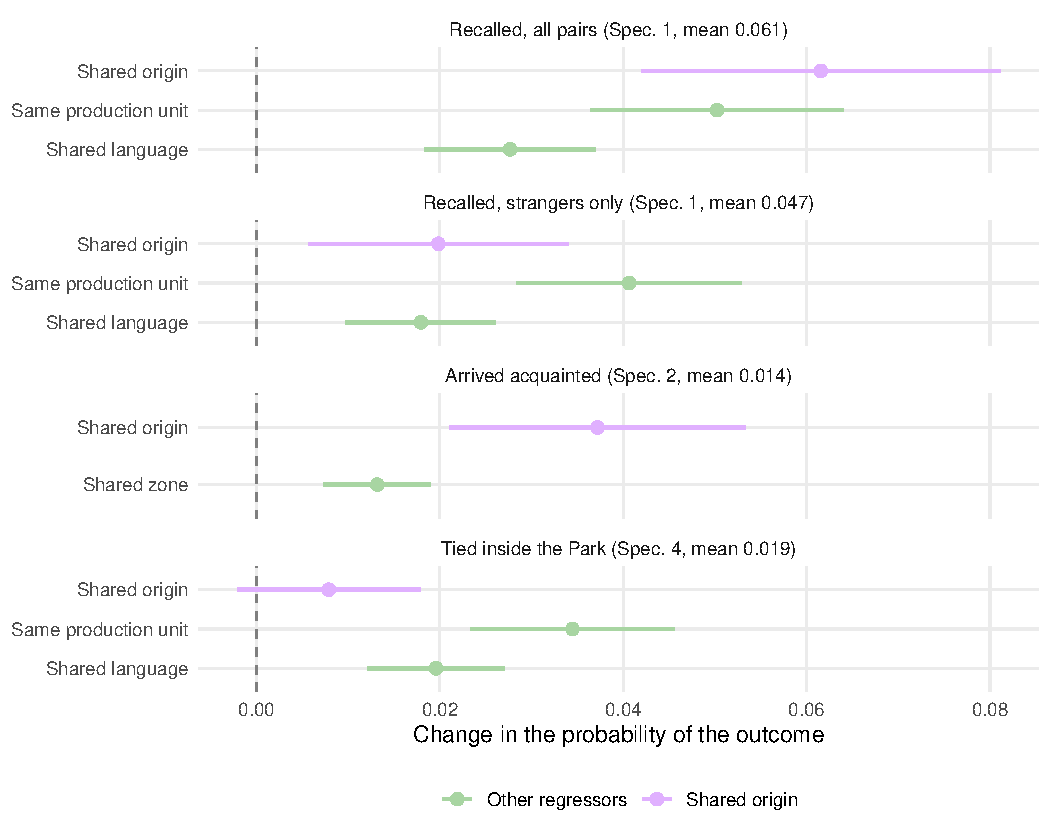
\includegraphics[width=0.85\textwidth]{../figures/fig_channels}
\fignote{Coefficients from Specification 1 on both of its samples, then Specifications 2 and 4, with 95\% confidence intervals. The four panels have different outcomes or samples, and different base rates, printed in each panel heading, but one common horizontal axis: the coefficients are all in probability points and rescaling each panel to its own base would make the panels incomparable, which is the comparison the figure exists to make.}
\end{figure}

\begin{table}[h!]
\centering
\caption{Specifications 2 to 4 - whether two workers are tied}
\label{tab:tie_formation}
\small% GENERATED by "21 analysis - channels.R" - do not edit by hand.
\begin{tabular}{lcccc}
& \shortstack{\textit{(2, inherited}\\\textit{ties)}} & \shortstack{\textit{(3, new ties)}} & \shortstack{\textit{(4, new ties,}\\\textit{same woreda)}} & \shortstack{\textit{(4, new ties,}\\\textit{same zone)}} \\
\dmidrule
Shared origin & 0.037*** & --- & 0.008 & --- \\
 & (0.008) &  & (0.005) &  \\
Shared zone & 0.013*** & --- & --- & 0.010*** \\
 & (0.003) &  &  & (0.003) \\
Same production unit & --- & 0.025*** & 0.034*** & 0.035*** \\
 &  & (0.004) & (0.006) & (0.006) \\
Shared language & --- & 0.011*** & 0.020*** & 0.018*** \\
 &  & (0.002) & (0.004) & (0.004) \\
\midrule
Sample & all pairs & strangers & strangers & strangers \\
Fixed effects & batch & batch & worker, alter & worker, alter \\
Observations & 19{,}522 & 19{,}239 & 19{,}239 & 19{,}239 \\
Mean of the outcome & 0.014 & 0.019 & 0.019 & 0.019 \\
MDE (80\% power) & --- & --- & 0.014 & 0.008 \\
\bottomrule
\end{tabular}

\fignote{Standard errors clustered on both members of the pair. *** 1\%, ** 5\%, * 10\%.}
\end{table}
\bigskip
\FloatBarrier

\noindent \underline{\textit{Specification 5: Exclusion}} \\[0.4em]
When considering a survey respondant of majority background, a minority is named \pnChanExclDeltaOutPp{} percentage points less often on the region definition ($\delta = \pnChanExclDeltaOut{}$, $p = \pnChanExclDeltaOutP{}$) and \pnChanExclLangDeltaOutPp{} points less often on the language definition ($\delta = \pnChanExclLangDeltaOut{}$, $p = \pnChanExclLangDeltaOutP{}$). Neither are powered nor significant. However, when the respondant is a minority worker herself, the penalty reverses into a significant premium of $\pnChanExclDeltaIn{}$ by region and $\pnChanExclLangDeltaIn{}$ by language (Table~\ref{tab:exclusion}). \\

\begin{table}[h!]
\centering
\caption{Specification 5 - whether a worker is refused}
\label{tab:exclusion}
\small% GENERATED by "21 analysis - channels.R" - do not edit by hand.
\begin{tabular}{lcc}
& \shortstack{\textit{(region)}} & \shortstack{\textit{(language)}} \\
\dmidrule
Receiver is minority & 0.005 & 0.005 \\
 & (0.004) & (0.004) \\
$\times$ namer is minority too & -0.031*** & -0.047*** \\
 & (0.010) & (0.013) \\
\midrule
Estimated on & dyads & dyads \\
Fixed effects & batch & batch \\
Observations & 19{,}522 & 19{,}522 \\
MDE (80\% power) & 0.010 & 0.011 \\
\bottomrule
\end{tabular}

\fignote{\textit{Region} defines minority as birth outside the Sidama region, \textit{language} as not speaking Sidamigna. Coefficients are $\delta$, so a positive number means the receiver is named \textit{less}. Standard errors clustered on both members of the pair. *** 1\%, ** 5\%, * 10\%.}
\end{table}
\bigskip


\clearpage
\parhead{Intensive margin}

\noindent \underline{\textit{Specification 6: Depth}} \\[0.4em]
\noindent Tie tenure is associated with deeper ties. Inherited co-hire ties carry \pnMuxDepthCohireInh{} layers on average, against \pnMuxDepthCohireNew{} for ties formed inside the Park (Table~\ref{tab:depth_cohire}). \\[-0.6em]

\noindent Shared origin does not deepen a tie. I get \pnMuxOriginCohire{} on the co-hire roster ($p = \pnMuxOriginCohireP{}$) and \pnMuxOriginGn{} in the general network ($p = \pnMuxOriginGnP{}$, Table~\ref{tab:depth_gn}). Both are negative and both are significant at the 5\% level or better. They also survive the kin and friend controls of column (3).  Interacting shared origin with vintage (tie inheritance) is not conclusive. \\[-0.6em]
 
 \noindent Thus, conditional on knowing someone at all, workers show no preference for their co-villagers. A shared woreda is associated with a narrower relationship rather than a richer one. What predicts the depth is whether they are related or friends to the alter. Kin and friends carry substantially more than acquaintances on the co-hire roster (\pnMuxKinCohire{} for kin), and somewhat less in the general network (\pnMuxKinGn{}).\\[-0.6em]
 
 \noindent Note that these estimates are limited by power\footnote{The co-hire column rests on \pnMuxOriginInhCellCohire{} same-woreda ties formed inside the Park. The vintage coefficient is identified only from workers reporting ties of both vintages (\pnMuxVintTiesCohire{} ties on the co-hire roster, \pnMuxVintTiesGn{} ties in the general network). Only \pnMuxPostCohire{} co-hire ties were formed after HIP, against \pnMuxPostGn{} general-network ones.}. Most workers are absorbed by the fixed effect and do not contribute to the estimate. \\

\begin{table}[h!]
\centering
\caption{Specification 6 - what makes a co-hire tie deep}
\label{tab:depth_cohire}
\small% GENERATED by "23 analysis - multiplexity.R" - do not edit by hand.
\begin{tabular}{lcccc}
& \shortstack{\textit{(6, no worker}\\\textit{FE)}} & \shortstack{\textit{(6, worker FE)}} & \shortstack{\textit{(6, + kin and}\\\textit{friend)}} & \shortstack{\textit{(6, +}\\\textit{origin~$\times$~vintage)}} \\
\dmidrule
Tie predates HIP & 0.41*** & 0.80*** & 0.61*** & 0.63*** \\
 & (0.06) & (0.17) & (0.18) & (0.18) \\
Shared birth woreda & -0.02 & -0.53** & -0.48* & -0.04 \\
 & (0.09) & (0.23) & (0.25) & (0.27) \\
Same woreda $\times$ pre-HIP & --- & --- & --- & -0.55 \\
 &  &  &  & (0.36) \\
Shared language & 0.05 & 1.03* & 0.81 & 0.82 \\
 & (0.15) & (0.53) & (0.51) & (0.51) \\
Same production unit & -0.06 & 0.14 & 0.16 & 0.16 \\
 & (0.06) & (0.17) & (0.16) & (0.16) \\
Kin & --- & --- & 0.86*** & 0.91*** \\
 &  &  & (0.29) & (0.28) \\
Friends & --- & --- & 0.84*** & 0.86*** \\
 &  &  & (0.16) & (0.15) \\
\midrule
Worker fixed effects & no & yes & yes & yes \\
Ties & 476 & 249 & 249 & 249 \\
Workers & --- & 117 & 117 & 117 \\
\bottomrule
\end{tabular}

\fignote{Standard errors clustered on both members of the pair. *** 1\%, ** 5\%, * 10\%.}
\end{table}
\clearpage

\noindent \underline{\textit{Specification 7: Vintage}} \\[0.4em]
\noindent  The  most common tie in the roster (workplace break, \pnMuxBreaksPrevCohire{}\% of ties) is not more likely to be associated with inherited ties. As expected, being a general network member is negatively associated with workplace ties. An alter known before HIP is markedly less likely to be someone the worker takes breaks with (\pnMuxBreaksGn{}), and more likely to be someone she would turn to for a large expense (\pnMuxLargeExpGn{}). This is consistent with the general network being at the village of origin (Table~\ref{tab:vintage_layers}, Figure~\ref{fig:layer_vintage}).

\begin{table}[h!]
\centering
\caption{Specification 7 - which layers an inherited tie carries}
\label{tab:vintage_layers}
\small% GENERATED by "23 analysis - multiplexity.R" - do not edit by hand.
\begin{tabular}{lcc}
\textit{layer} & \shortstack{\textit{(7, co-hire ties)}} & \shortstack{\textit{(7, general network)}} \\
\dmidrule
rosca ekub & 0.031 (0.038) & 0.021 (0.018) \\
assistance (out) & 0.037 (0.038) & 0.106*** (0.025) \\
large expenses (out) & 0.040 (0.028) & 0.099*** (0.021) \\
borrow money (out) & 0.060 (0.074) & 0.065** (0.031) \\
large expenses (in) & 0.077 (0.059) & 0.309*** (0.023) \\
call or text & 0.094 (0.084) & 0.162*** (0.035) \\
friends & 0.097 (0.111) & 0.058 (0.039) \\
workplace breaks & 0.105 (0.087) & -0.505*** (0.042) \\
meet outside work & 0.173* (0.091) & 0.085** (0.037) \\
job search & 0.188** (0.086) & 0.120*** (0.029) \\
borrow money (in) & 0.210** (0.087) & 0.063* (0.037) \\
assistance (in) & 0.213*** (0.061) & 0.187*** (0.031) \\
advice personal decision & 0.250*** (0.094) & 0.151*** (0.028) \\
navigate hawassa & 0.301*** (0.083) & 0.126*** (0.030) \\
commute & 0.321*** (0.083) & -0.130*** (0.040) \\
\midrule
Ties & 399 & 3{,}029 \\
\bottomrule
\end{tabular}

\end{table}

\begin{figure}[h!]
\centering
\caption{Specification 7 - which layers an inherited tie carries}
\label{fig:layer_vintage}
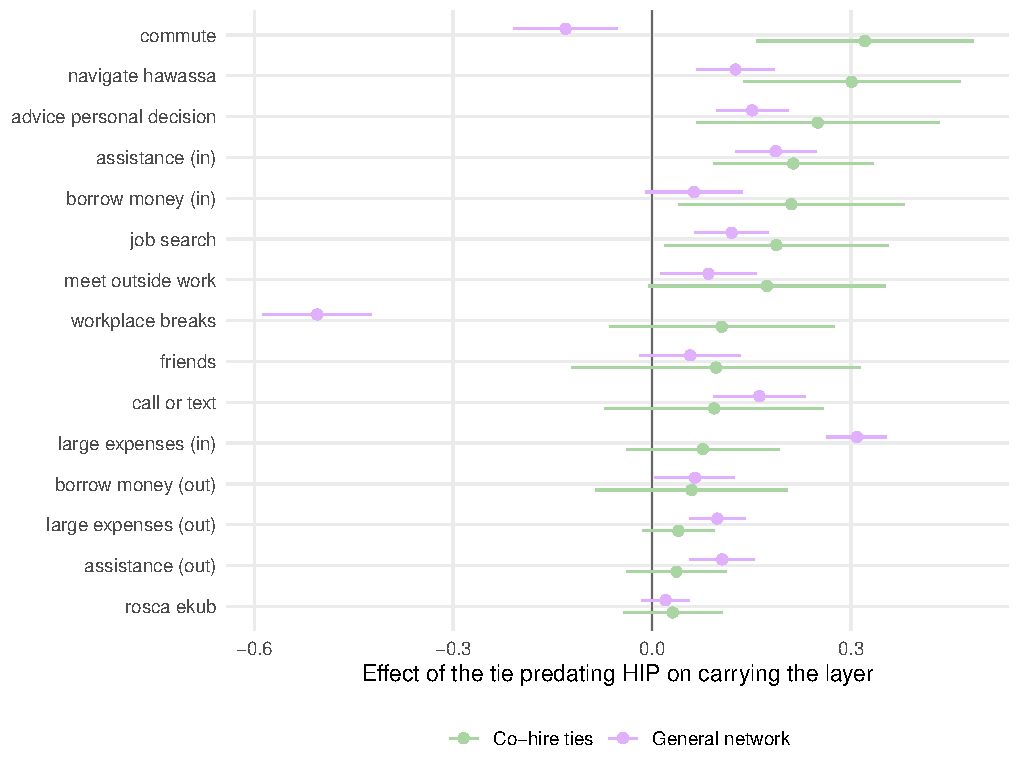
\includegraphics[width=0.7\textwidth]{../figures/fig_layer_vintage}
\end{figure}
\clearpage

\noindent \underline{\textit{Specification 8: Multiplexing}} \\

\noindent Specification 6 said a co-villager tie is not deeper. This one asks whether it is differently shaped (\textit{i.e.} if it loads on different functions), and it appears to be.\\[-0.6em]

\noindent In the general network, ties tilted toward money and help and away from company (Table~\ref{tab:layers_gn}). A same-woreda tie is more likely to be someone the worker would turn to for a large expense (\pnLayerLargeExpGn{}) and less likely to be someone she takes her workplace breaks with (\pnLayerBreaksGn{}), these consistent with the general network being away from HIP.\\[-0.6em]

\noindent Origin here masks kin - \pnLayerKinShareGn{}\% of the \pnLayerOriginTiesGn{} same-origin ties are kin, against \pnLayerKinShareGnNon{}\% of the rest. Fitted side by side the origin profile and the kinship profile trace nearly the same shape across the fifteen layers (correlation \pnLayerProfileCorrGn{}). 

\noindent Holding kinship, vintage and co-residence fixed , the money layers disappear. Two co-villagers who are not relatives are less likely to be workplace company, whether taking breaks (\pnLayerBreaksGnCtrl{}) or finding one's way around Hawassa (\pnLayerNavigateGnCtrl{}, the one coefficient the controls barely move), but more likely to be named friends (\pnLayerFriendsGnCtrl{}, against \pnLayerFriendsGn{} before). I read this as the co-villager relation being an affective one rather than a practical one, once the family tie is taken out (Figure~\ref{fig:layer_origin}). \\[-0.6em]

\noindent The co-hire roster shows no comparable reshaping, but with only \pnLayerOriginTiesCohire{} of \pnLayerTiesCohire{} co-hire ties sharing a woreda this is an underpowered null (Table~\ref{tab:layers_cohire}). \\[-0.6em]
\bigskip

\begin{table}[h!]
\centering
\caption{Specification 8 - what a shared origin does to what a general-network tie is for}
\label{tab:layers_gn}
\small% GENERATED by "22 analysis - layer design.R" - do not edit by hand.
\begin{tabular}{lcc}
\textit{layer} & \shortstack{\textit{(8, no controls)}} & \shortstack{\textit{(8, + kinship, vintage, co-residence)}} \\
\dmidrule
advice personal decision & 0.034** (0.014) & -0.005 (0.016) \\
borrow money (in) & 0.010 (0.015) & 0.012 (0.017) \\
large expenses (in) & 0.203*** (0.015) & 0.017 (0.016) \\
job search & 0.001 (0.014) & -0.007 (0.016) \\
navigate hawassa & -0.042*** (0.014) & -0.047*** (0.015) \\
commute & -0.066*** (0.015) & 0.003 (0.018) \\
meet outside work & -0.058*** (0.015) & 0.008 (0.017) \\
call or text & 0.027* (0.015) & 0.026 (0.017) \\
workplace breaks & -0.147*** (0.016) & -0.055*** (0.017) \\
friends & -0.061*** (0.016) & 0.052*** (0.018) \\
assistance (in) & 0.081*** (0.014) & 0.004 (0.015) \\
rosca ekub & -0.015 (0.011) & 0.001 (0.012) \\
borrow money (out) & -0.035*** (0.013) & -0.002 (0.014) \\
large expenses (out) & 0.070*** (0.011) & 0.004 (0.012) \\
assistance (out) & -0.001 (0.011) & -0.010 (0.012) \\
\midrule
Joint test, $\chi^2(14)$ & 286.63*** & 33.33*** \\
Ties & 3{,}030 & 3{,}030 \\
\hspace{1em}of which shared origin & 1{,}952 & 1{,}952 \\
Tie-by-layer observations & 45{,}450 & 45{,}450 \\
\bottomrule
\end{tabular}

\fignote{Standard errors clustered on the pair. *** 1\%, ** 5\%, * 10\%.}
\end{table}

\begin{table}[h!]
\centering
\caption{Specification 8 - what a shared origin does to what a co-hire tie is for}
\label{tab:layers_cohire}
\small% GENERATED by "22 analysis - layer design.R" - do not edit by hand.
\begin{tabular}{lcc}
\textit{layer} & \shortstack{\textit{(8, no controls)}} & \shortstack{\textit{(8, + kinship, vintage, co-residence)}} \\
\dmidrule
advice personal decision & 0.046 (0.044) & 0.042 (0.047) \\
borrow money (in) & 0.050 (0.048) & 0.009 (0.050) \\
large expenses (in) & -0.023 (0.031) & -0.008 (0.033) \\
job search & 0.003 (0.049) & 0.023 (0.052) \\
navigate hawassa & -0.001 (0.047) & -0.044 (0.047) \\
commute & 0.047 (0.047) & -0.003 (0.049) \\
meet outside work & 0.123** (0.048) & 0.058 (0.049) \\
call or text & -0.076 (0.048) & -0.092* (0.051) \\
workplace breaks & 0.002 (0.050) & 0.044 (0.053) \\
friends & -0.014 (0.050) & 0.022 (0.051) \\
assistance (in) & -0.023 (0.038) & -0.018 (0.039) \\
rosca ekub & -0.019 (0.031) & 0.025 (0.033) \\
borrow money (out) & -0.038 (0.037) & -0.026 (0.040) \\
large expenses (out) & -0.024 (0.027) & 0.003 (0.025) \\
assistance (out) & -0.052** (0.023) & -0.034 (0.026) \\
\midrule
Joint test, $\chi^2(14)$ & 18.31 & 14.28 \\
Ties & 652 & 652 \\
\hspace{1em}of which shared origin & 90 & 90 \\
Tie-by-layer observations & 9{,}780 & 9{,}780 \\
\bottomrule
\end{tabular}

\fignote{Standard errors clustered on the pair. *** 1\%, ** 5\%, * 10\%.}
\end{table}

\FloatBarrier

\begin{figure}[h!]
\centering
\caption{Shared origin, and what survives holding kinship fixed}
\label{fig:layer_origin}
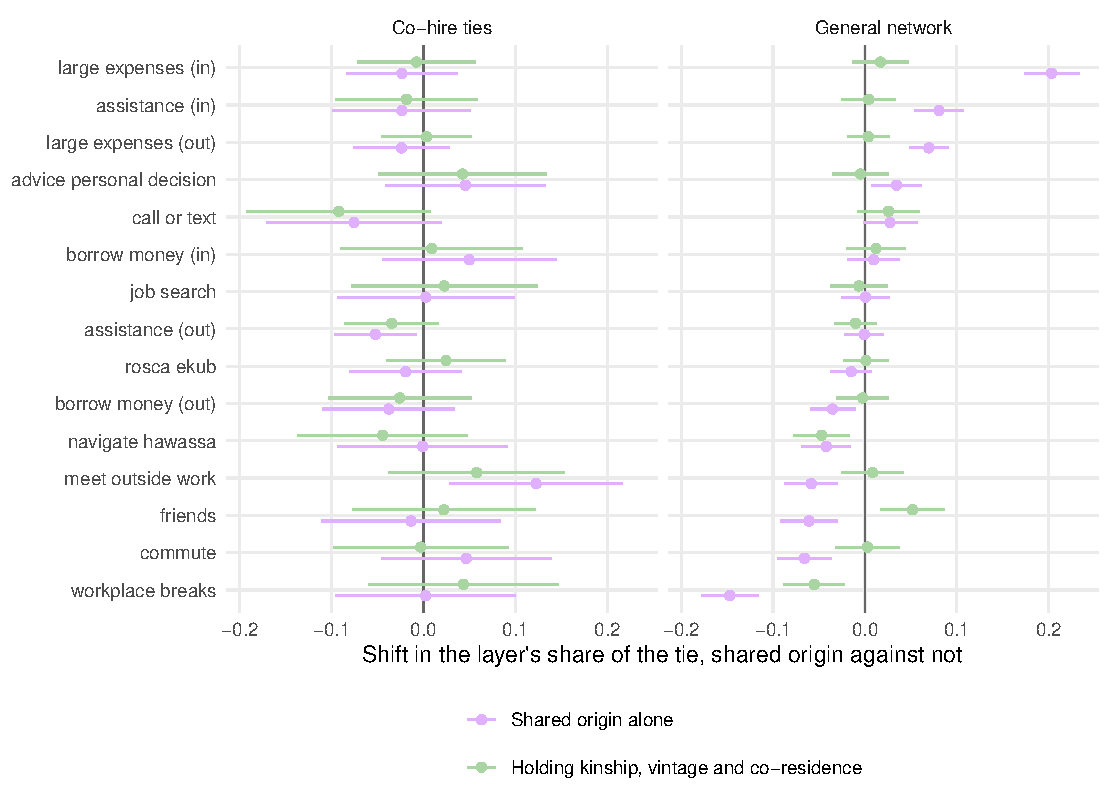
\includegraphics[width=0.95\textwidth]{../figures/fig_layer_origin}
\end{figure}
\clearpage
